\chapter{系统软件平台设计}
低功耗海洋传感器集成系统的软件平台设计,主要包括系统管理与配置模块、能源管理与控制模块、数据采集与通信模块、数据存储与回收模块四大部分。系统配置与管理模块实现了系统和测试、管理人员的外部交互,通过该模块进行参数配置,包括系统时间设置、定时设置、工作模式设置等功能。能源管理与控制模块主要负责控制系统的工作状态,不同的工作状态下对电源进行管理。数据采集与通信模式则是完成与传感器的交互,实现了对传感器数据的收发。数据存储与回收模块对采集数据进行了有效的保存。

\section{软件设计基本原则}
(1)高内聚、低耦合是系统软件设计遵循的基本原则。系统按需求划分为不同的功能模块,各模块各司其职保持高独立性,同时按照需求提供相应的接口函数。

(2)由于系统服役环境的影响,系统软件设计优先考虑系统的功耗和稳定性,确保系统在高稳定状态下以最高的效率、最低的功耗完成分配的任务。 

(3)软件设计需考虑可扩展性,即对未来功能的可扩展性,当系统增加新 功能时,对现有系统软件的结构和代码改动尽可能小。

(4)低功耗海洋传感器集成系统软件设计需实现相应的调试函数,可通过该函数进行单独指令测试、参数配置和系统状态监控,确保联调时各个系统的工作状态可视化。

\section{系统管理与配置模块}
系统管理与配置模块主要作用是,管理人员通过该模块对整个系统的参数进行配置,比如系统第一次运行时,设置系统参数和定时采样的时间等。
\subsection{系统主流程}
当电路板上电或复位后,系统首先进行初始化,包括串口初始化、SPI初始化、RTC初始化、各个外设模块初始化以及用于逻辑控制的普通I/O口模式配置初始化等。接着系统会读取后备寄存器并对相应的变量进行初始化赋值,后备寄存器存储着系统的重要变量,后备寄存器不会因为掉电而丢失数据,后备区域供电引脚VBAT脚采用混合供电的方式,由CR2110纽扣电池和3.3V电池同时供电,确保RTC的运行和防止后备寄存器数据丢失。系统初次运行可通过预留的调试接口进行系统参数的配置,包括系统时钟、定时时间等参数。然后系统进入低功耗模式,并等待闹钟中断和串口中断唤醒CPU,完成中断请求任务后系统再次进入低功耗模式。流程图如图~\ref{fig:系统流程图}所示。

\begin{figure*}[ht]
    \centering
	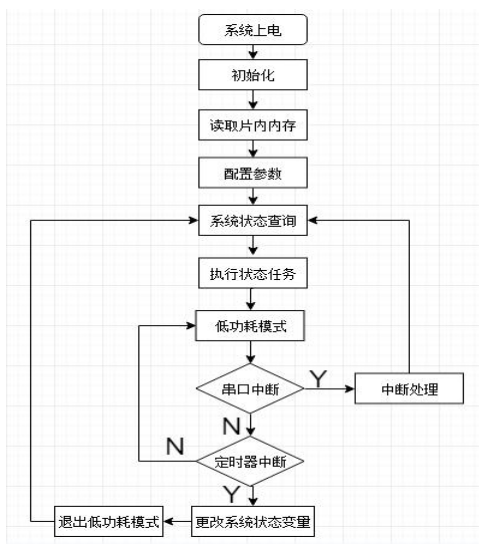
\includegraphics[width=0.6\textwidth]{fig/系统流程图.png}
	\caption{系统流程图}
	\label{fig:系统流程图}
\end{figure*}

\subsection{系统配置}
在电子电路设计中将串口一用串口转USB芯片转化成了用于系统调试的USB接口。该接口主要用作系统参数的配置,还可以通过拟定指令查询系统的运行状态、提取备份数据等。

系统时间设置和定时时间设置都是微处理器通过SPI总线访问高精度实时钟芯片DS3234来实现的。时间和日历数据由写入适当的寄存器字节来设置和初始化。时间和日历寄存器的内容是BCD码格式。DS3234可以运行在24或者12小时模式。微处理器访问DS3234内部SRAM数据,进行读写时钟数据,即可获取到系统时钟。定时时间设置是通过DS3234的闹钟中断来实现的,设置闹钟时间为系统时间加上定时时长,每次系统时间与闹钟时间一致时,触发闹钟中断(DS3234的INT/SQW低电平有效)。系统的工作可分为两种,一种是正常工作模式,一种是定时模式,在定时模式下,系统会监测定时时间,达到定时时间则开始数据采集,在采样的周期之间系统会自动进入低功耗模式,可以下达Wake指令进行唤醒,也可以下达Sleep指令让系统随时进入低功耗模式。每次系统参数配置会保存下来,如需对参数进行清除可以下达Empty指令。系统配置指令如表~\ref{tab:系统配置指令}所示。
\begin{table*}[ht]
\caption{系统配置指令}
  \label{tab:系统配置指令}
\centering
    \begin{tabular}{|c|c|}
        \toprule
 {\bf 指令}&{\bf 说明}  \\      
%\bf表示字体加粗
        \hline
[TM=YYMMDD hhmmss]& \tabincell{c}{配置系统时间,YY代表 年,MM代表月,\\DD代表日,hh代表时,mm代表分,ss代表秒。} \\
%需要分行的单元格的语句用\tabincell{c}{所填写第一行内容\\第二行内容···},可以根据需要换行,也不限定换多少行。
        \hline
[cmd\_mod\_x]& \tabincell{c}{改变系统工作状态,x为0系统配置为正\\常模式,x为1系统配置为定时模式} \\
        \hline
SetTM=YYMMDD hhmmss& \tabincell{c}{配置定时时间,YY代表年,MM代表月,\\DD代表日,hh代表时,mm代表分,ss代表秒。} \\
        \hline
Empty& \tabincell{c}{清空系统的参数和flash} \\
     \hline
Wake& \tabincell{c}{系统唤醒} \\
     \hline
Sleep& \tabincell{c}{系统进入低功耗} \\
        \bottomrule
    \end{tabular}
\end{table*}
\subsection{独立看门狗设计}
为防止系统因外界环境干扰或不可预见的逻辑条件造成程序跑飞陷入死循环~\cite{hjm},软件上使用了独立看门狗设计,当独立看门狗IWDG被激活后,IWDG的计数器开始向下递减计数,当IWDG的计数器的值递减到0时,系统便会复位,为保证系统正常工作,必须在IWDG的计数器的值递减到0之前,重新给IWDG的计数器赋值。独立看门狗启动之后,在程序中便不能关闭,必须在规定时间内喂狗,否则将会产生一个复位信号导致系统重启。

独立看门狗这种设计的时钟源频率为40kHz,它采用LSI内部低速时钟,这种配置使得系统主时钟出现错误时,该时钟依旧能保持正常运行。独立看门狗初始化函数中,配置IWDG\_PR寄存器的值为0x06,即预分频系数prer设置为6,配置IWDG\_RLR寄存器的值为0xfff,即重装在值 rlr为 4095。溢出时间计算公式如式\ref{eq:times}:
\begin{equation}
\begin{split}
T_{out}=[(4\times(2^{prer})) \times rlr] /40 ms
\end{split}
\label{eq:times}
\end{equation}  

公式中T指代看门狗溢出时间,prer指代独立看门狗时钟预分频系数,rlr为独立看门狗的重装载值,可计算溢出时间为26.208s。由于RC振荡器频率不是一个精准的40kHz,实际值和理论值会有一定的偏差,故在系统软件设计中,必须预留足够的时间进行喂狗操作。当系统进入低功耗模式时,为防止系统因未喂狗而导致重启,软件上设置内部RTC闹钟中断,配置中断间隔为10s,在闹钟中断处理函数中会更改系统状态变量从而进入系统自检状态,在系统自检中进行喂狗操作。

\section{能源管理与控制模块}
能源管理与控制模块块的主要功能是,最大限度地减少电流的损耗,微处理器长期控制整个能源管理系统,在外部设备不工作时,切断其能源供应,并微处理器自身进入低功耗模式,系统时钟切换成低速外部时钟。
\subsection{电源管理设计}
低功耗海洋传感器集成系统在程序设计上,根据设定的采样周期获取海洋生态环境数据。系统各个外部部件的实际工作时间是很有限的,在外部部件的待机时间内,通过电源管理设计尽可能的减少待机时间功耗,用以达到低功耗设计的目标。

电源管理设计可以控制海洋传感器设备处于断电状态并且微处理器进入低功耗状态,这是控制系统能源消耗最佳的措施。上节介绍了定时时间的设置,当系统到达定时时间意味着要开始采集任务了。通过定时中断将微处理器从低功耗状态下唤醒,唤醒之后,微处理器命令给海洋传感器上电,然后海洋传感器接受下达的采集命令,最后海洋传感器进行数据采集任务。传感器的电源供应选择了可控式的DC/DC模块,其中的ctrl引脚连接到了微处理器的IO口上。

默认设置下,微处理器控制DC/DC模块处于断电的状态。在定时中断函数中,给对应ctrl引脚的IO口置位,即可完成给海洋传感器的上电。微处理器在设定的时刻可以通过中断来从低功耗模式进入到活跃模式,在周期性的活跃模式之间,微处理器皆会在LMP3低功耗模式下运行。电源管理流程图如图~\ref{fig:电源管理流程图}所示。
\begin{figure*}[ht]
    \centering
	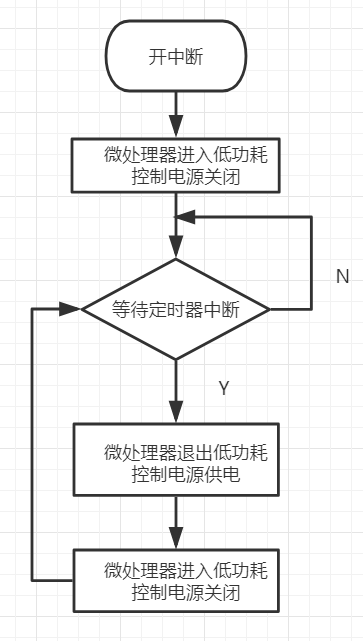
\includegraphics[width=0.5\textwidth]{fig/电源管理流程图.png}
	\caption{电源管理流程图}
	\label{fig:电源管理流程图}
\end{figure*}
\subsection{时钟切换设计}
微处理的功耗受到很多因素的影响,其中系统的运行频率是非常关键的影响要素。在关闭外部设备供电的情况下,MCU的功耗就主要取决于其系统时钟。

一般情况下,设计应选择尽可能小的运行频率。前文的硬件平台介绍提到,系统的时钟来源主要有两个:高速外部晶振电路(16MHz)和DS3234提供的低速32768Hz时钟。采用低速时钟作为系统运行频率,无疑会节省更多的能源损耗,但是考虑到系统处于活动模式下,微处理要参与完成众多的任务,比如与海洋传感器通信进行数据采集任务、与TF卡通信完成数据存储任务等,主系统MCLK为32768Hz时,系统的性能会大大的降低。所以根据系统实际应用的情况,要考虑到时钟的切换,即在系统正常工作的活跃状态下,要把微处理器的主系统时钟MCLK从LFXT1(外部低速晶振)切换到LFXT2(外部高速晶振),进入到低功耗模式下,微处理器只需维持基本的功能,等待中断将其唤醒,此时将系统时钟从高速切换回低速时钟。

% MSP430内部时钟图解如图~\ref{fig:MSP430时钟框架}所示。

% \begin{figure*}[ht]
%     \centering
% 	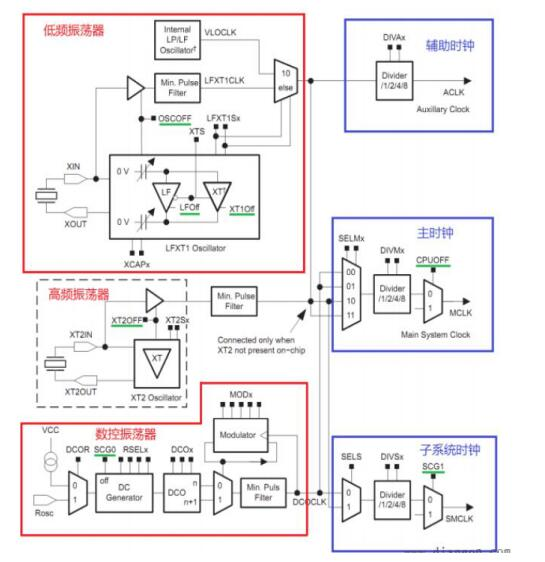
\includegraphics[width=0.7\textwidth]{fig/MSP430时钟框架.jpg}
% 	\caption{MSP430时钟框架}
% 	\label{fig:MSP430时钟框架}
% \end{figure*}

系统开启时,默认设置初始时钟为内部的DCO时钟。同时把XT1和XT2的功能都禁止了。但是DCO是内部集成的数字频率振荡器,其一内部的时钟频率不稳定,这会影响到系统的定时等功能,其二频率可能达不到性能要求。所以通常在使用时,都会切换到外部的晶体振荡器时钟。在本系统设计中,会涉及到这三种时钟的切换。比如,系统一上电后,初始时钟为默认的内部DCO时钟,然后进入低功耗模式下,时钟切换为外部低速时钟(32768Hz),需要执行采集任务时,系统处于活跃模式,时钟切换为高速外部时钟(16MHz)。

系统时钟主要通过修改BCSCTL1和BCSCTL2两个寄存器来配置。这两个寄存器的详细说明如图~\ref{fig:BCSCTL1寄存器}和图~\ref{fig:BCSCTL2寄存器}所示。
\begin{figure*}[ht]
    \centering
	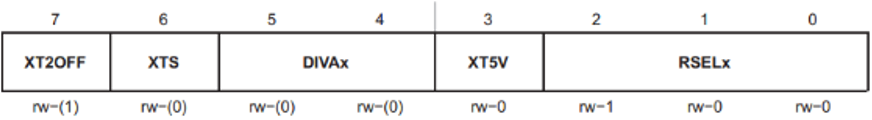
\includegraphics[width=1\textwidth]{fig/BCSCTL1寄存器.png}
	\caption{BCSCTL1寄存器}
	\label{fig:BCSCTL1寄存器}
\end{figure*}

XT2OFF:是否关闭高频振荡器。0开;1关。

XTS:选择低速晶体振荡器的工作方式。0为低;1为高。

\begin{figure*}[ht]
    \centering
	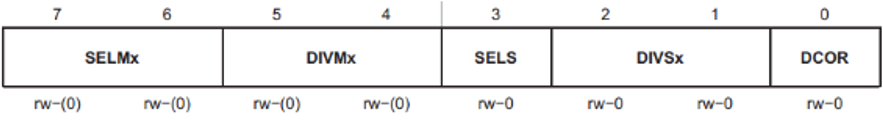
\includegraphics[width=1\textwidth]{fig/BCSCTL2寄存器.png}
	\caption{BCSCTL2寄存器}
	\label{fig:BCSCTL2寄存器}
\end{figure*}
SELMx:主系统时钟来源选择。

SELS:子系统时钟来源选择。

时钟来源要切换到外部时钟上去,一般需要进行几个步骤:

1)打开外部晶体振荡器,因为默认配置下XT1和XT2的功能是被禁止的。

2)清除晶体振荡器失效标志OFIFG标志。

3)等待50us,等待外部晶体振荡器工作。

4)监测晶振振荡器失效标志OFIFG标志,如果它没有失效,则外部晶体振荡器工作正常。

切换为XT2的程序代码实例如下:

\begin{lstlisting}[language=c++]
void ClokInit{
BCSCTL1&=~XT2OFF; //首先打开外部晶体振荡器。
 do{
    IFG1&=~OFIFG; //清除晶体振荡器失效标志OFFIFG标志
    for(int i=0xFF;i>0;i--); //等待50us,等待晶体振荡器正常工作
    }while((IFG1&OFIFG));//当OFFIFG等于0的时候结束,说明其正常工作。
BCSCTL2 |= SELM_2;
BCSCTL2 |= SELS;   //选择XT2时钟
}
\end{lstlisting}

\subsection{实时钟RTC设计}
低功耗海洋传感器集成系统的低速外部时钟直接是由高精度时钟芯片DS3234来提供的。一方面在电子电路设计中舍弃了外部晶振电路,简化电路设计和节省能源消耗;另外一方面为系统提供更加准确的时钟,这对于按点的电源管理和多参数数据的准同步都有重要的作用。通过设置DS3234的控制/状态寄存器来使能32KHz方波输出,控制/状态寄存器如图所示。

\begin{figure*}[ht]
    \centering
	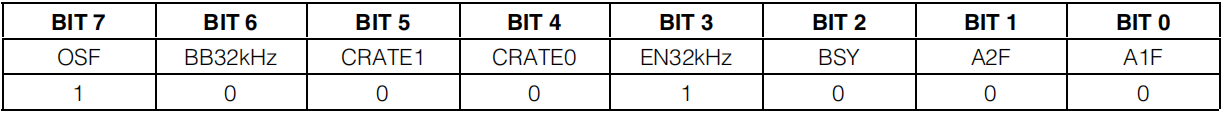
\includegraphics[width=1\textwidth]{fig/控制状态寄存器.png}
	\caption{控制状态寄存器.png}
	\label{fig:控制/状态寄存器}
\end{figure*}
位3是32KHz输出的使能,给位3置位时,输出一个32768Hz的方波输入。具体的操作是,微处理器通过SPI方式给控制状态寄存器(Ox0F)地址写入。
\section{数据采集与通信模块}
数据采集与通信模块的主要作用是,实现微处理器与海洋传感器之间的信息交互,比如微处理给传感器下达控制指令,传感器返回数据和状态信息等。
\subsection{串口中断软件设计}
数据采集与通信模块采集数据的方式是通过串口中断的方式实现的,同时预留的的调试接口都采取了中断的方式,当中断发生时,首先会对数据有效性进行判断,海洋观测数据以"*"开头,调试串口的数据以"["开头。每采集到一帧有效的海洋观测数据时,回复"[sendok]"表明接收成功并更改系统状态变量为Sava\_Data即数据存储状态,在主循环的系统状态检测中进入数据存储状态进行数据存储,存储成功后,相应的记录存储帧数的计数器将会加1,待发送数据帧数计数器也会加1,在系统自检状态检测到待发送数据帧数时将更改系统状态变量为Send\_Data即数据发送状态,在下一次系统状态检测中进入数据发送状态发送数据,数据发送成功时,对应的待发送数据帧数减1,已发送数据帧数加1,并将变量更新到系统状态表中并写入片内Flash的信息存储区,以便系统复位后对该信息重新获取。对于调试接口的数据,系统则对指令数据进行解析并执行对应的指令任务,任务完成后系统又进入到低功耗模式等到下一次中断的发生。串口中断程序流程图如图~\ref{fig:串口中断流程图}所示。

\begin{figure*}[ht]
    \centering
	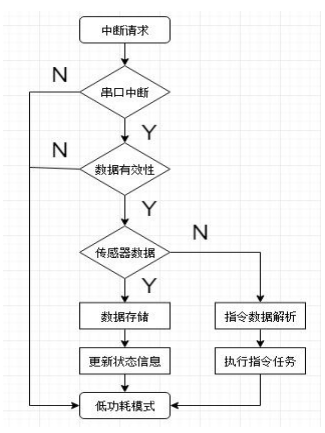
\includegraphics[width=0.7\textwidth]{fig/串口中断流程图.png}
	\caption{串口中断流程图}
	\label{fig:串口中断流程图}
\end{figure*}

\subsection{拓展串口软件设计}
针对微处理器现有的串口数量不足的问题,采用串口拓展芯片WK2124进行串口数量的拓展。微处理器是有多余的SPI总线接口的,所以在芯片选型时,选用可以实现SPI拓展4个串口功能的WK2124。SPI是串行外设接口,本质上是一个移位寄存器,将数据串行的输出到外围设备。通信原理主要以主从方式进行工作,可以实现一主多从工作模式。在本文中主要采用了主模块进行工作,即微处理器为主设备,串口拓展芯片为从设备,通常以四根线相连接进行通信,如表格~\ref{tab:SPI工作线}所示。

\begin{table}[htb]
  \centering\small
  \caption{SPI工作线}
  \label{tab:SPI工作线}
\begin{tabular}{|c|c|c|}
\hline
\multicolumn{2}{|c|}{\bf 名称}                  & {\bf 说明}                         \\ \hline
\multicolumn{2}{|l|}{MISO}                  & \multicolumn{1}{|c|}{主设备输入,从设备输出}                \\ \hline
\multicolumn{2}{|l|}{MOSI}                  & \multicolumn{1}{c|}{主设备输出,从设备输入}                \\ \hline
\multicolumn{2}{|l|}{SCLK}                  & \multicolumn{1}{c|}{时钟信号,由主设备产生}                         \\ \hline
\multicolumn{2}{|c|}{CS}                  & \multicolumn{1}{c|}{片选信号线,由主设备控制}                     \\ \hline
\end{tabular}
\end{table}

串口拓展芯片所通信的时钟主要由微处理器通过SCK引脚提供,再经由SPI的CS线选中需要进行数据传输任务的从设备。SPI的数据传输有着不同的总线协议模式,微处理器与WK2124必须配置相同的参数并使用相同的模式才能进行正常的通信,主要有两个参数决定SPI的传输方式:时钟极性和时钟相位,为芯片选择寄存器中的CPOL和CPHA位~\cite{2009zw},分别可取0或1,组成四种SPI工作模式,如表格~\ref{tab:SPI总线协议模式}所示。

%\newcommand{\tabincell}[2]{\begin{tabular}{@{}#1@{}}#2\end{tabular}}  
%表格自动换行
\begin{table*}[ht]
\caption{SPI总线协议模式}
  \label{tab:SPI总线协议模式}
\centering
    \begin{tabular}{|c|c|c|}
        \toprule
 {\bf SPI Mode}&{\bf CPOL} & {\bf CPHA}  \\      
%\bf表示字体加粗
        \hline
[0]& {0} & {0}\\
%需要分行的单元格的语句用\tabincell{c}{所填写第一行内容\\第二行内容···},可以根据需要换行,也不限定换多少行。
        \hline
[1]& {0} & {0}\\
\hline
[2]& {1} & {1}\\
\hline
[3]& {1} & {0}\\
        \bottomrule
    \end{tabular}
\end{table*}
SPI的四种工作模式区别主要是根据SCLK跳变沿进行数据采样~\cite{2006zxj},即在于是在SCLK的哪一位置进行数据传输任务,详细的工作原理和时序图分析不再赘述,具体可以参考数据手册和相关文档。

主设备MSP430F5438A微处理器通过SPI接口访问从设备WK2124,读取拓展串口采集的数据。WK2124工作在SPI同步串行通信的从机模式下,支持SPI模式0标准。为实现主机和WK2124的通信,在主机端需要设置CPOL=0(SPI时钟极性选择位),CPHA=0(SPI时钟相位选择位)。写FIFO操作,即给海洋传感器发送指令,先写入一个命令字节(Command Byte),随后写入相应的数据字节,FIFO地址自动增加。读FIFO操作,即接收海洋传感器采集数据,先写入一个命令字节(Command Byte),随后芯片SDOUT线上会返回相应的数据字节。FIFO地址自动增加。相关通信的流程图如图~\ref{fig:SPI通信流程图}所示。
\begin{figure*}[ht]
    \centering
	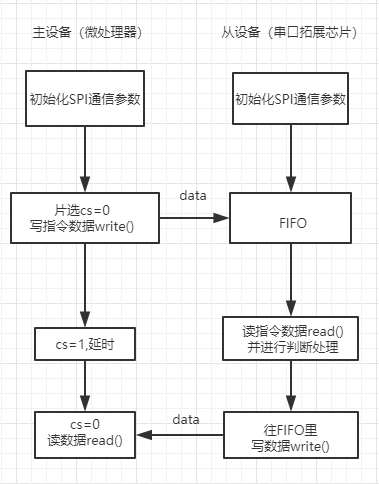
\includegraphics[width=0.6\textwidth]{fig/SPI通信流程图.png}
	\caption{SPI通信流程图}
	\label{fig:SPI通信流程图}
\end{figure*}

\subsection{传感器通信软件设计}
数据采集与通信模块最终的目标就是,通过微处理器本身的串口和拓展串口实现与海洋传感器的通信。各个海洋传感器与微处理器系统之间的通信方式主要是依靠RS232、RS285已经AML传感器本身的通信协议,中间主要是经过了相关电平信号的转换,所采集的数据才直接进入到微处理器当中。微处理器对于传感器下达的指令根据传感器类型的不同而不同,主要是对传感器的采样频率、时间校准、数据格式等进行相关配置,一般包括唤醒、开始采样和结束采样等命令,其中对于传感器的命令格式和详细配置在前面的章节均已介绍,下面主要是对命令转发到传感器的数据协议进行制定,如表格~\ref{tab:控制指令通信协议}所示。

%\newcommand{\tabincell}[2]{\begin{tabular}{@{}#1@{}}#2\end{tabular}}  
%表格自动换行
\begin{table*}[ht]
\caption{控制指令通信协议}
  \label{tab:控制指令通信协议}
\centering
    \begin{tabular}{|c|c|c|c|c|}
        \toprule
 {\bf 数据标号}&{\bf 字段名称} & {\bf 数据类型}& {\bf 数据长度} & {\bf 备注说明} \\      
%\bf表示字体加粗
        \hline
{\bf 1}& {包头} & {ASCII码}& {1 Byte} & \tabincell{c}{“*”-数据包的开始 }\\
\hline
%需要分行的单元格的语句用\tabincell{c}{所填写第一行内容\\第二行内容···},可以根据需要换行,也不限定换多少行。
{\bf 2}& {控制命令} & {ASCII码}& {不等} & \tabincell{c}{控制命令的内容和长度\\ 依据对应的传感器进行选取}\\
        \hline
{\bf 3}& {校验位} & {8 位无符号整数}& {1 Byte} & \tabincell{c}{对命令进行校验,默认为 0xff}\\
        \hline
{\bf 4}& {包尾} & {ASCII码}& {1 Byte} & \tabincell{c}{“*”-数据包的结束}\\
        \bottomrule
    \end{tabular}
\end{table*}

命令通过 RS232或485下发到传感器后,传感器会执行相关的指令,同时不同的传感器会将采集回来的数据传送到微控制器,其数据量比较大,且接收到的数据需要进行解析处理,所以需要单独分类,可以根据提前预定好的串口ID号来区分传感器,然后提取数据。对于返回数据量较大的传感器将预先设定足够大的缓冲区,可以通过自定义的队列结构暂存数据,然后按照时间节点进行传送。将按照表格~\ref{tab:数据包结构}的数据包结构进行数据采集。

%\newcommand{\tabincell}[2]{\begin{tabular}{@{}#1@{}}#2\end{tabular}}  
%表格自动换行
\begin{table*}[ht]
\caption{数据包结构}
  \label{tab:数据包结构}
\centering
    \begin{tabular}{|c|c|c|c|c|c|c|}
        \toprule
 {\bf 包头}&{\bf 相关信息} & {\bf 间隔}& {\bf 数据} & {\bf 间隔}& {\bf 校验}& {\bf 包尾} \\      
%\bf表示字体加粗
        \hline
{*}& {数据类型-\#-ID-\#-" 时间"} & {\#}& {数据体} & {\#}& {校验位}& {*}\\
        \bottomrule
    \end{tabular}
\end{table*}

除了包含主要的数据体外,还包括包头包尾、ID号、时间等必要的信息,其中ID主要是针对串口来事先定义好的标号,以此来区分不同的传感器。

\section{数据存储与回收模块}
数据储存与回收模块的主要作用是,系统的较长时间内采集的海洋水文数据都能够完整地进行存储,以便系统设备打捞上来后对数据进行回收备份。
\subsection{TF卡程序设计}
本次设计牺牲传输速率而选择了简便、速率稍低的SPI连接方式。上文介绍了SPI相关使用软件设计,本部分从TF卡程序设计进行阐述。

本次设计采用SPI总线与TF卡进行通信,需要首先进行的就是设置TF卡为SPI总线模式。具体的操作方法是:片选信号在复位命令来的时候处于有效的电平。由于TF内部供电电压上升需要一定的时间,这个时间大概是64个时钟左右,之后TF卡又要花费10时钟来进行卡同步,所以发送CMD0命令之前必须要等待74个时钟。TF卡初始化分为以下几个步骤:

1)初始化SPI接口及相关IO。通过SPI连接SD卡,所以先要初始化MCU的SPI接口,以及相关IO。

2)上电延时(>74个CLK)。 

3)卡复位(CMD0),进入IDLE状态。发送CMD0时,CS必须为低电平,使得SD卡进入SPI模式。

4)发送CMD8,检查是否支持SD卡2.0协议。

5)采用不同协议检查SD卡。

6)片选取消,结束初始化。

TF卡初始化流程图如图~\ref{fig:TF卡初始化流程}所示。
\begin{figure*}[ht]
    \centering
	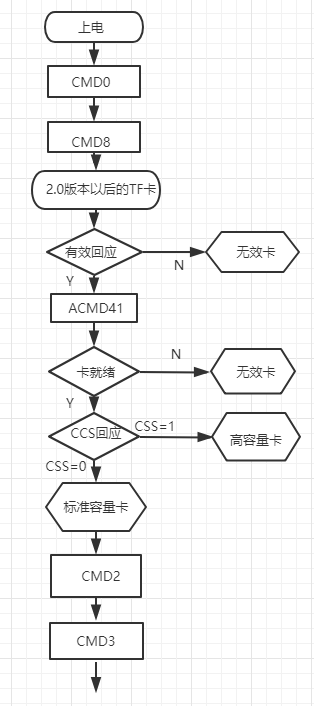
\includegraphics[width=0.5\textwidth]{fig/TF卡初始化流程.png}
	\caption{TF卡初始化流程}
	\label{fig:TF卡初始化流程}
\end{figure*}
\subsection{FATFS文件系统设计}
系统应用TF卡,需要文件系统管理进行协助。在众多的文件系统中,本文选择使用FATFS文件系统来管理TF卡。FATFS是一个完全用广泛认可的C语言编写的免费开源文件系统模块,硬件平台独立性使他优于其他文件模块,在移植到 8051、PIC、AVR、SH、Z80、H8、ARM等系列单片机时有较好的适用性,只需少量简单的修改。它支持多种存储格式和多个存储媒介;支持多个文件的读写操作。

FATFS的许多优点,以及它在软件开发上免费、开源的原则,使得FATFS应用非常广泛。FATFS模块的层次结构如图~\ref{fig:FATFS模块层次结构图}所示:

\begin{figure*}[ht]
    \centering
	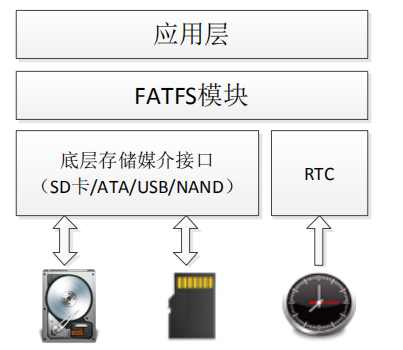
\includegraphics[width=0.5\textwidth]{fig/FATFS模块层次结构图.png}
	\caption{FATFS模块层次结构图}
	\label{fig:FATFS模块层次结构图}
\end{figure*}

如图~\ref{fig:FATFS模块层次结构图}所示,应用层直接给用户提供了丰富的接口函数,将它置于顶部,帮助用户简单使用而无需关注内部结构和协议等具体细节。中间层对文件的读写协议进行具体的要求,对于使用者不做修改要求,若需使用,将头文件进行引用便可。底层存储媒介接口需要进行代码编写移植的工作。

在进行FATFS移植之前,要做一些准备工作。在其官网获取FATFS软件包最新资源,解压获取到的资源包,得到doc和src两个文件夹。FATFS文件系统结构如图~\ref{fig:FATFS文件系统结构}所示。

\begin{figure*}[ht]
    \centering
	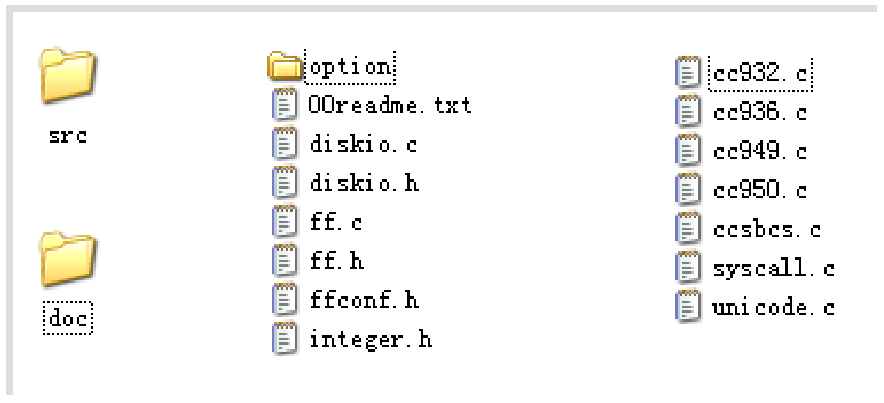
\includegraphics[width=0.7\textwidth]{fig/FATFS文件系统结构.png}
	\caption{FATFS文件系统结构}
	\label{fig:FATFS文件系统结构}
\end{figure*}

doc里面主要是对FATFS的介绍,而src里面是源码。硬件层包括diskio.c和diskio.h。文件系统的API层包括ff.c和ff.h。用户对ffcon.h和diskio.c进行修改配置,一般就能够完成移植的任务。ffconf.h里面包含了FATFS模块的所有配置信息和设置选项,可根据实际应用需求进行选择修改。diskio.c的主要功能是与底层硬件接口进行连接适配。这些文件的功能说明如表格~\ref{tab:FATFS文件系统包}所示。
%\newcommand{\tabincell}[2]{\begin{tabular}{@{}#1@{}}#2\end{tabular}}  
%表格自动换行
\begin{table*}[ht]
\caption{FATFS文件系统包}
  \label{tab:FATFS文件系统包}
\centering
    \begin{tabular}{|c|c|c|}
        \toprule
 {\bf 文件名}&{\bf 功能} & {\bf 说明} \\      
%\bf表示字体加粗
        \hline
 {ffconf.h}&{FATFS模块配置文件} & \tabincell{c}{需要根据需求\\来配置参数。} \\      
%\bf表示字体加粗
        \hline
 {ff.h}&{FATFS和应用模块公用的包含文件} & {不需要修改} \\      
%\bf表示字体加粗
        \hline 
 {ff.c}&{FATFS模块源码} & {不需要修改} \\      
%\bf表示字体加粗
        \hline
 {diskio.h}&{FATFS和disk I/O模块公用的包含文件} & {不需要修改} \\      
%\bf表示字体加粗
        \hline
{diskio.c}&{FATFS和disk I/O模块接口层文件} &\tabincell{c} {与平台相关的代码,\\需要用户根据存储介质来编写函数。} \\ 
%\bf表示字体加粗
        \hline
{interger.h}&{数据类型定义} & {与编译器有关。} \\ 
%\bf表示字体加粗
        \hline
{option文件夹}&{可选的外部功能(比如支持中文等)} & {根据应用环境} \\ 
        \bottomrule
    \end{tabular}
\end{table*}

移植FATFS文件系统的一般包括以下几个步骤:

1)数据类型:在integer.h里面去定义好数据的类型。这里需要了解你用的编译器的数据类型,并根据编译器定义好数据类型。

2)配置:通过ffconf.h配置FATFS的相关功能,以满足设计的需要。

3)函数编写:打开diskio.c,进行底层驱动编写,一般需要编写6个接口函数,如图~\ref{fig:diskio.c要实现的函数}所示。
\begin{figure*}[ht]
    \centering
	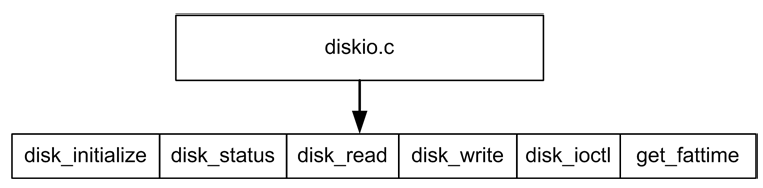
\includegraphics[width=0.7\textwidth]{fig/diskio.c要实现的函数.png}
	\caption{diskio.c要实现的函数}
	\label{fig:diskio.c要实现的函数}
\end{figure*}

通过软件设计部分将这六个函数一一实现,完成了对FATFS的移植之后,将可以在系统中正常的使用FATFS了。FATFS提供了很多API函数,在这里就不做过多的
赘述。建立好文件系统以后,首先建立一个数据文件夹(根据系统布放地点命名),然后根据日期来建立存储海洋水文数据的文件,每天生成一个TXT文件用来记录数据,如图~\ref{fig:水文数据文件}所示。
\begin{figure*}[ht]
    \centering
	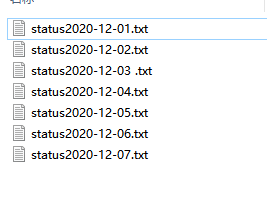
\includegraphics[width=0.5\textwidth]{fig/水文数据文件.png}
	\caption{水文数据文件}
	\label{fig:水文数据文件}
\end{figure*}

\section{本章小结}
在本章中主要针对低功耗海洋传感器集成系统的软件平台部分进行了详细的介绍,由于整个系统工作在海底环境,在软件设计上优先保障系统的低功耗性和 稳定性,首先介绍系统软件的设计原则,然后重点介绍和分析了四个功能模块的软件设计。